\documentclass{article}

% Packages
\usepackage[utf8]{inputenc} % Required for German umlauts
\usepackage{amsmath}
% SVG
\usepackage{svg}
% Bib
\usepackage[backend=biber]{biblatex}
\addbibresource{bib/bibliography.bib}
% Subimages
\usepackage{subfig}
% Geometry
\usepackage[left=2cm, right=2cm, top=2cm]{geometry}

%%
%% Custom commands
%%

%
% Tikz Setup
%
\usepackage[customcolors]{hf-tikz}

\tikzset{style green/.style={
    set fill color=green!50!lime!60,
    set border color=white,
  },
  style cyan/.style={
    set fill color=cyan!90!blue!60,
    set border color=white,
  },
  style orange/.style={
    set fill color=orange!80!red!60,
    set border color=white,
  },
  hor/.style={
    above left offset={-0.15,0.31},
    below right offset={0.15,-0.125},
    #1
  },
  ver/.style={
    above left offset={-0.1,0.3},
    below right offset={0.15,-0.15},
    #1
  }
}

\author{Stanislaw Hüll}
\title{Student Research Project}
\date{2018-11-11}
\begin{document}

\maketitle

\section{Introduction}

  \subsection{Compressed Sparse Row Format}
    It is a widely used storage format for sparse matrices which does not make assumptions about the matrix's shape
    or its distribution of non-zero elements in contrast to other popular sparse matrix storage formats such as the
    the diagonal storage format or ELLPACK. It optimizes the storage requirements of general sparse matrices with
    respect to the naive coordinate format (COO) in that each non-zero's row index is no longer explicitly stored.

    The CSR format consists of three dense arrays:

    The values array stores the numerical value for each non-zero entry in the matrix while their column index is stored
    in the associated column-index array. A third array, the row-pointer array, encodes the beginning of each row's
    section within the values and column-index arrays, i.e. it stores the offset of each row's first non-zero element
    into the two previous arrays. Thus the CSR format optimizes the storage requirements of general sparse matrices with
    respect to the naive coordinate format (COO) in that each-nonzero's row index is no longer explicitly stored,
    shrinking the size of the third array from one entry per non-zero element to a single entry per row.

    % CSR format example

\begin{equation}\label{fig:csr_example}
  \left(\begin{array}{cccc}
    \tikzmarkin[hor=style green]{row0}  3 & 0 & 4 & 0 \tikzmarkend{row0} \\
    \tikzmarkin[hor=style cyan]{row1}   0 & 0 & 0 & 0 \tikzmarkend{row1} \\
    \tikzmarkin[hor=style orange]{row2} 0 & 0 & 7 & 8 \tikzmarkend{row2} \\
  \end{array}\right)
\end{equation}


    By convention, the non-zeros are stored row-wise in ordered fashion from left to right implying that each row's
    section within the column-index array is sorted in ascending fashion. Additionally, the row-pointer array contains
    an additional element denoting the total number of non-zero elements in the structure. Note that sometimes a
    different nomenclature is utilized in the existing literature, referring to the arrays as A (values), JA
    (column-indices) and IA (row-pointers), respectively \cite{sparskit}.

    The CSR format's salient feature is its direct access to a row's non-zero elements' values and column indices making
    it particularly well suited for matrix-vector-multiplication utilizing a conventional row-by-column computation
    scheme. Aside of this feature storing the non-zero elements row by row as opposed to column by column is, to a
    certain degree, arbitrary and thus exist numerical libraries and toolkits such as the Eigen C++ library
    \cite{eigen:website} or the Harwell-Boeing sparse matrix collection \cite{harwell-boeing} which utilize the CSR
    format's conjugate, the compressed sparse column format (CSC), as their default means of representing sparse
    matrices.

  \subsection{Structured Grid Matrices}

    Structured grid computations are ubiquitously used for physical simulations for computational fluid dynamics,
    electrodynamics and astrophysics.  In contrast to unstructured grids the regularity inherent to structured grids
    allows for very efficient numerical treatment, such that even in cases where sufficiently complex geometries
    prohibit the decomposition of the target domain into a single overarching structured grid the domain is often
    tesselated into an unstructured configuration, with the tiles being filled by independent structured grids
    \cite{Badcock2000}.

    To derive an approximate solution to a physical system's set of partial differential equations
    the PDEs are discretized on the structured grid by approximating the differential operators by algebraic
    expressions. A promiment example is the Cartesian finite-difference approximation of the Laplacian operator.
    The discretization step yields a linear problem $A x = b$ in which the right-hand side $b$ depends only on the
    boundary conditions and is thus known.

    (((TODO))) The solution of this linear system by iterative means requires that, starting at an initial guess $x_0$,
    a stencil operation is applied to each node, i.e. its new value is determined by a weighted sum of the current
    values of its adjacent nodes. Which nodes are considered adjacent depends on the approximation of the differential
    operators, but in general the pattern is symmetric with respect to the node in question while the individual weights
    of the weighted sum might change from node to node. The stencil corresponding to the finite-difference Laplacian is
    the symmetric 5-point or 7-point stencil for 2D or 3D grids, respectively.

    The stencil operation across the grid can be expressed in terms of a matrix-vector multiplication, where
    the vector contains the grid nodes' function values and the matrix is the grid's adjacency matrix, whose non-zero
    entries encode the adjacency relation of the stencil across the whole matrix and whose numeric values are the
    weighted sum's weights. These adjacency matrices have a very characteristic structure, whose exact shape depends on
    the type of boundary condition underlying the physical system's PDEs and on the stencil's geometry. In general, they
    are symmetric and consist of as many diagonals as there are nodes in the stencil. The diagonals are almost fully
    dense with exceptions arising at positions corresponding to nodes at the grid's boundaries, where the
    adjacency pattern is disturbed by missing nodes as in the case of Dirichlet boundary conditions. Adjacency matrices
    are symmetric and have one row and column per node in the grid.

    \begin{figure}[htbp]
  \centering
  \includesvg{adj_mat}
  \caption{svg image}
\end{figure}


    TODO: Bisher nur finite difference, was ist mit FEM?

    Arise as finite difference adjacency matrices from discretization of elliptic type PDE (SPARSKIT 7.1)
      and structured mesh finite element matrices.
    Are (locally) structured.
    "Almost" diagonal --> DIA not the best. [Godwin2013: p9!!!]

\section{Three-fold compressed sparse row}

// TODO: Section with nomenclature
  - structure, pattern, ...

  Evidently, representing a structured grid's adjacency matrix using the regular CSR format is highly suboptimal, as it
  has no means of capturing the obvious repetetiveness of the structure. While at first glance the diagonal format seems
  to be an appealing choice for the types of matrices introduced in the previous section, real-life problems produce
  matrices which are only locally structured, i.e. they contain multiple fully structured sections corresponding to the
  multiple structured grid regions of the overall heterogeneous domain mentioned above, which need not be aligned in
  a way to produce a diagonal structure at all. Thus a more flexible approach is taken adapting the CSR format.

  Additionally, utilizing a CSR-like format keeps open the possibility to eventually tackle adjacency matrices of
  unstructured grids.

  This section introduces the data layout and storage scheme of the three-fold compressed sparse row format which allows
  for the utilization of certain compression mechanisms explained thereafter. Finally, the algorithms required to
  perform common arithmetic operations are presented.

  \subsection{Data layout and storage scheme}

    The basic motive of this work is to leverage the regularity inherent in structured grid adjacency matrices. The vast
    majority of the matrix's rows share a common column index pattern. Their non-zero elements occur at fixed offsets
    with respect to the row's first non-zero element's position.

      ((( TODO: Bild )))

    It is cruicial to observe that, in the most general case, the index patterns' regularity is not shared by the
    non-zero elements' numerical values. While two or more rows may share the same pattern their corresponding values
    need not be similar to each other at all and, possibly, even vice versa. To prevent that a lack of common regularity
    impedes optimizing the storage requirements of one or the other it is hence necessary to decouple the representation
    of a row's column index positions from the representation of its numerical values. The C3SR format accounts for this
    circumstance and maintains separate data structures for the patterns and values.

    //TODO Erst colindices einführen, dann values und darauf hinweise, dass VS redundant ist, falls keine values
    compression erwünscht ist.

    The values are represented by two arrays which utilize the CSR's basic idea of storing all relevant data in an
    array (V) and managing a separate start-index array (VS) pointing each row's section's first element.

      ((( TODO: Bild. Einfache matrix mit values )))

    The column indices are stored abiding by the same principle with the additional detail that each row's column
    indices are decomposed into the absolute index of the row's first non-zero element, which is referred to as the
    row's 'peg', and the relative offsets of the remaining non-zeros' column indices with respect to the peg index.
    This introduces a degree of freedom whose usefulness will become evident in the context of compression. Thus the
    column indices are encoded into an array storing the patterns (J), another array storing the peg index (JP)
    and an index pointer array (JS) into J in the same way that VS relates to V.

      ((( TODO: Bild )))

    A sixth and final array (RS) is used to encode the number of non-zeros in each row of the matrix in order to know
    the size of the row's section within the pattern array and the values array. The RS array is an immediate copy of
    the CSR format's row-pointer array.  While the respective start index-pointer arrays store the section's first
    element's index they cannot encode the size of the section. Prior to compressing the size of a row can indeed be
    retrieved from the corresponding start index-pointer array in the same way the CSR format's row size may be
    retrieved from the row-pointer array by taking the difference between the row's entry and its successor, however,
    this requires that the row's sections are stored contiguously in the arrays and this property is lost during
    compression as will be explained in the next section.

    Summarizing the data organization of the C3SR format:
    \begin{itemize}
      \item Data representing the matrix's non-zero elements: V, VS
      \item Data representing non-zero elements' column indices: J, JP, JS
      \item Array containing information about the row sizes: RSS
    \end{itemize}

  \subsection{Compression mechanism}

    Using this storage scheme the column index information may be compressed by removing duplicate patterns from J and
    updating the start-index pointers JS of such duplicate rows to point the start of the corresponding unique section
    within J.

      ((( TODO: Bild )))

    The information about the non-zeros' values can be compressed in precicely the same way: Duplicate sections within V
    corresponding to different rows with identical values are removed and the corresponding start pointers are updated.

    In theory, the compression of patterns and values are orthogonal operations and if the overall goal were to minimize
    the storage requirement of a C3SR object in memory the best advice would be to exploit duplication in the matrix as
    much as possible. However, efficient arithmetic requires considerations going beyond maximum compression such as
    parallel performance and parallel scalability implying that the implementation must heed the principles of
    data locality and independence of tasks in the control flow of the algorithm.

    (((TODO: Partitioning during compression + stable- and non-stable values compression)))

    Note that this section avoids reasoning about low-level details for the sake of clarity. Tweaks such as the omission
    of each pattern's first value, which is always zero or mapping two partially matching rows' sections within J onto
    each other for a little gain in storage space optimization are considered implementation details are are not discussed
    here.

  \subsection{Algorithms}

    Stencil operation is applied multiple times during the solution, thus matvecmult speed is critical.

    \subsubsection{Matvecmult}
      improves locality (--> Performance)

    \subsubsection{Element access A[i;j]}
      binary lookup

\section{Performance Benchmarks}
  Measure performance in terms of (1) data compression ratio and (2) arithmetic performance (matvecmult)

  \subsection{Generation of structured grid adjacency matrices as test matrices}

    For the purpose of gauging the performance test matrices are created in CSR format which are then converted to C3SR
    format and compressed. These matrices resemble the structure of the structured grid matrices introduced above and
    are created by iterating through a 3D grid of fixed integral dimensions X, Y, Z and applying a given stencil
    which encodes the desired adjacency relationship. Nodes requested by the stencil but missing from the grid, i.e.
    nodes on the grid's outer borders are omitted, i.e. their corresponding entries in the adjacency matrix carry a zero
    which is equivalent to Dirichlet-type boundary conditions.

    The matrix's non-zero entries' numeric values are obtained from evaluating a sinusoidal function at the geometric
    center point $\vec{r} = (x, y, z)$ inbetween the two nodes in question whereby each Cartesian component $x, y, z$ is
    scaled by its coordinate's span $X, Y, Z$. An additional offset serves to prevent that entries in the matrix
    correponding to adjacent nodes according to the stencil incidentally evaluate to 0. The function utilized is
    $$W(x,y,z; n_x, n_y, n_z) = 2 + \sum \limits_{d \in \{x,y,z\}} \sin{\frac{d}{d_{\text{max}}} \cdot \pi \cdot n_d} $$
    where $n_x, n_y, n_z$ are periodicity parameters for each dimensions.

    Note that $n_d = 0 \Leftrightarrow \partial_d W(\vec{r}) \equiv 0$, introducing a periodicity in the corresponding
    dimension $d$. This feature is utilized to create periodicity in the matrix's values.

    (((Example of matrix + Computation of nonzeros)))

  \subsection{Data compression}

    This plot compares the number of array elements required in the C3SR format to store a fully structured matrix's column index information (green curve) against the baseline size of the equivalent CSR format matrix's column index array (red curve) depending on the partition size utilized for the structural compression. The C3SR format's recorded number of elements comprises the sum of the sizes of the J, JP and JS arrays, respectively. The RS array and the CSR format's row-pointer array are left out of the consideration as they are identical in size. The underlying $50 \times 50 \times 50$ grid contains $125000$ nodes to which the symmetric 7-pt stencil is applied. The numerical values of the matrix are of no concern for its structure.

    The C3SR format's diminishing storage requirements are caused solely by J (blue curve) as JS and
    JP are constant in size, each containing $125000$ elements, one per matrix row. The size of J
    exhibits an inverse linear relationship to the partition size, as can be inferred from the
    straight line's gradient in the double logarithmic plot. This is due to the fact that large
    grids mainly consist of inner nodes whose corresponding rows in the matrix all share the same pattern. Hence the overwhelming majority of partitions' column index information will condense to 7 elements within J (and one element per row for JS and JP) irrespective of the partition size with exceptions arising only around the few border nodes and their corresponding rows.

    The minimum size of J is determined by the matrix's unique patterns which correspond to 8 corner
    nodes a 4 adjacent nodes, 12 edge nodes a 5 adjacency nodes, 6 face nodes a 6 adjaceny nodes and
    the inner nodes with the full 7 adjacency nodes totalling $135$ entries. (TODO: Tikz 3d-draw
    representative of all nodes creating unique patterns).

    TODO: Ausreißer erklären.
    \begin{figure}[ht]
      \centering
      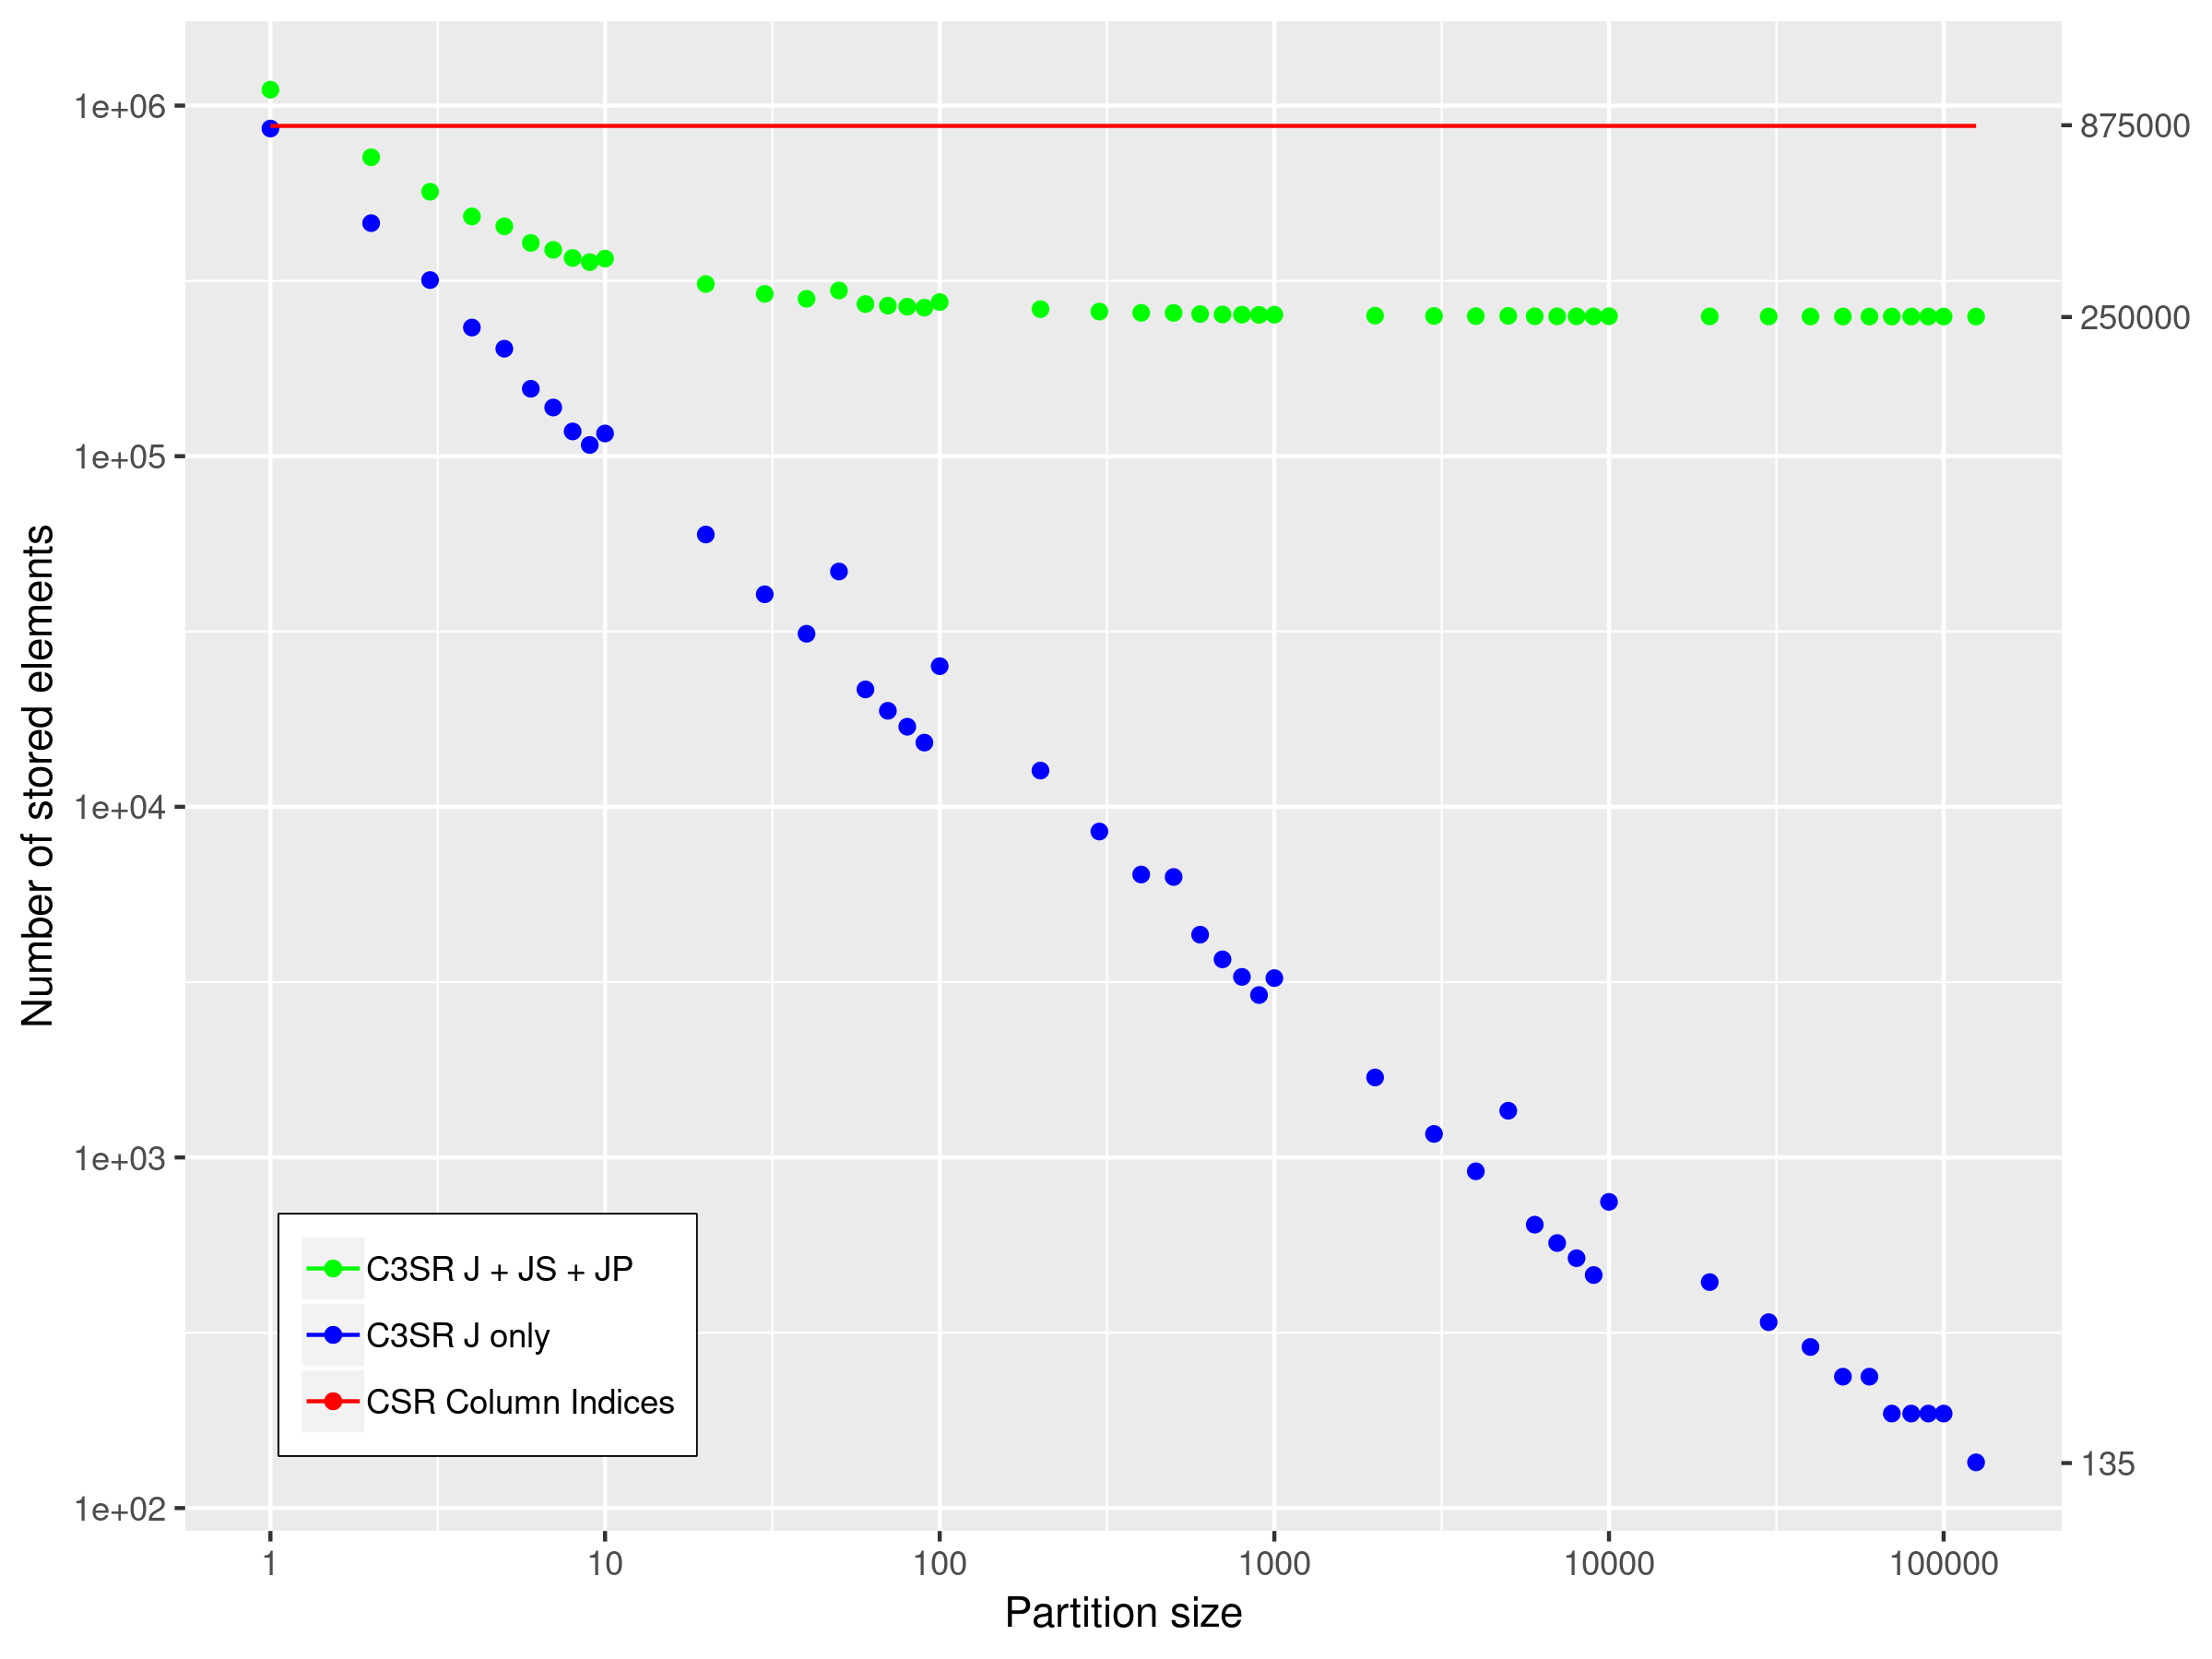
\includegraphics[width=0.8\textwidth]{fig/structural-compression}
      \caption*{TODO}
    \end{figure}

    //TODO: Structural compression mit interleaved matrices

  \subsection{Arithmetic Performance of Matrix-Vector Multiplication}

    This plot compares the number of array elements required in the C3SR format to store a fully structured matrix's column index information (green curve) against the baseline size of the equivalent CSR format matrix's column index array (red curve) depending on the partition size utilized for the structural compression. The C3SR format's recorded number of elements comprises the sum of the sizes of the J, JP and JS arrays, respectively. The RS array and the CSR format's row-pointer array are left out of the consideration as they are identical in size. The underlying $50 \times 50 \times 50$ grid contains $125000$ nodes to which the symmetric 7-pt stencil is applied. The numerical values of the matrix are of no concern for its structure.

    The C3SR format's diminishing storage requirements are caused solely by J (blue curve) as JS and
    JP are constant in size, each containing $125000$ elements, one per matrix row. The size of J
    exhibits an inverse linear relationship to the partition size, as can be inferred from the
    straight line's gradient in the double logarithmic plot. This is due to the fact that large
    grids mainly consist of inner nodes whose corresponding rows in the matrix all share the same pattern. Hence the overwhelming majority of partitions' column index information will condense to 7 elements within J (and one element per row for JS and JP) irrespective of the partition size with exceptions arising only around the few border nodes and their corresponding rows.

    The minimum size of J is determined by the matrix's unique patterns which correspond to 8 corner
    nodes a 4 adjacent nodes, 12 edge nodes a 5 adjacency nodes, 6 face nodes a 6 adjaceny nodes and
    the inner nodes with the full 7 adjacency nodes totalling $135$ entries. (TODO: Tikz 3d-draw
    representative of all nodes creating unique patterns).

    \begin{figure}[!ht]
      \centering
      \subfloat{
        \centering
        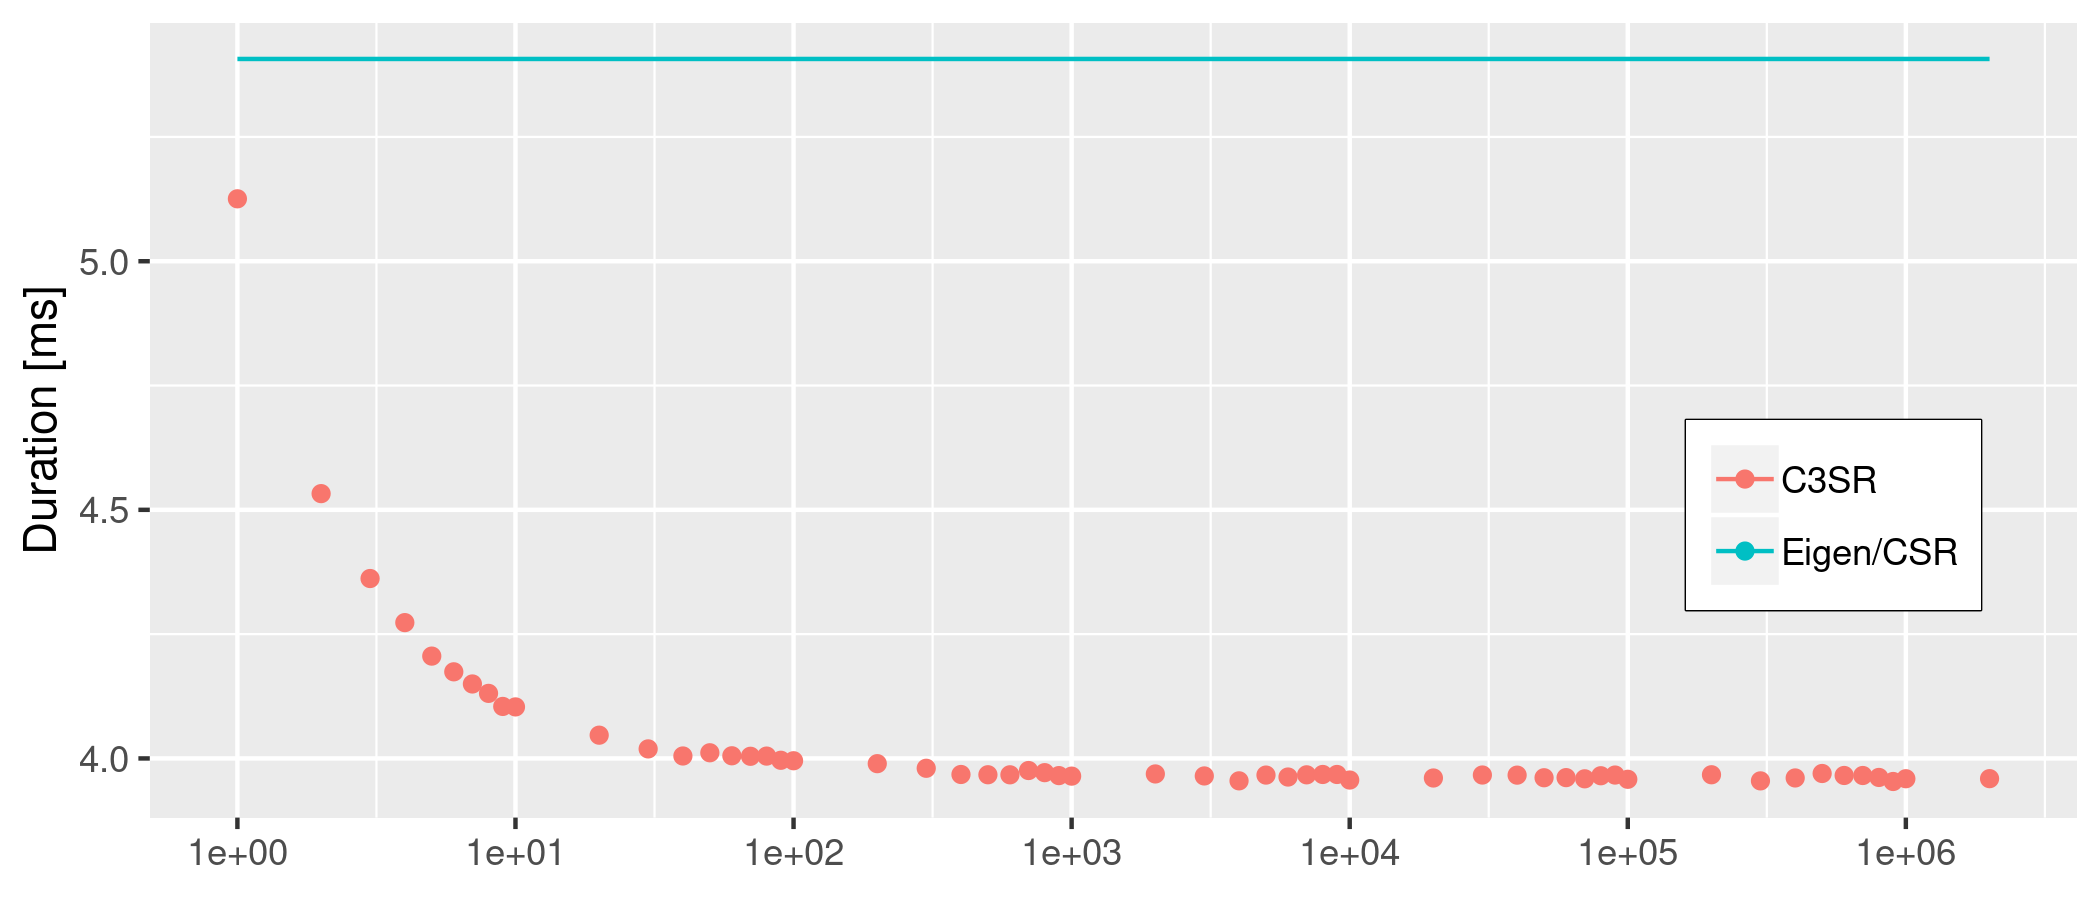
\includegraphics[width=0.9\textwidth]{assets/bench-matvecmult-structured-duration}
        \label{fig:bench-matvecmult-structured-duration}}\par
      \subfloat{
        \centering
        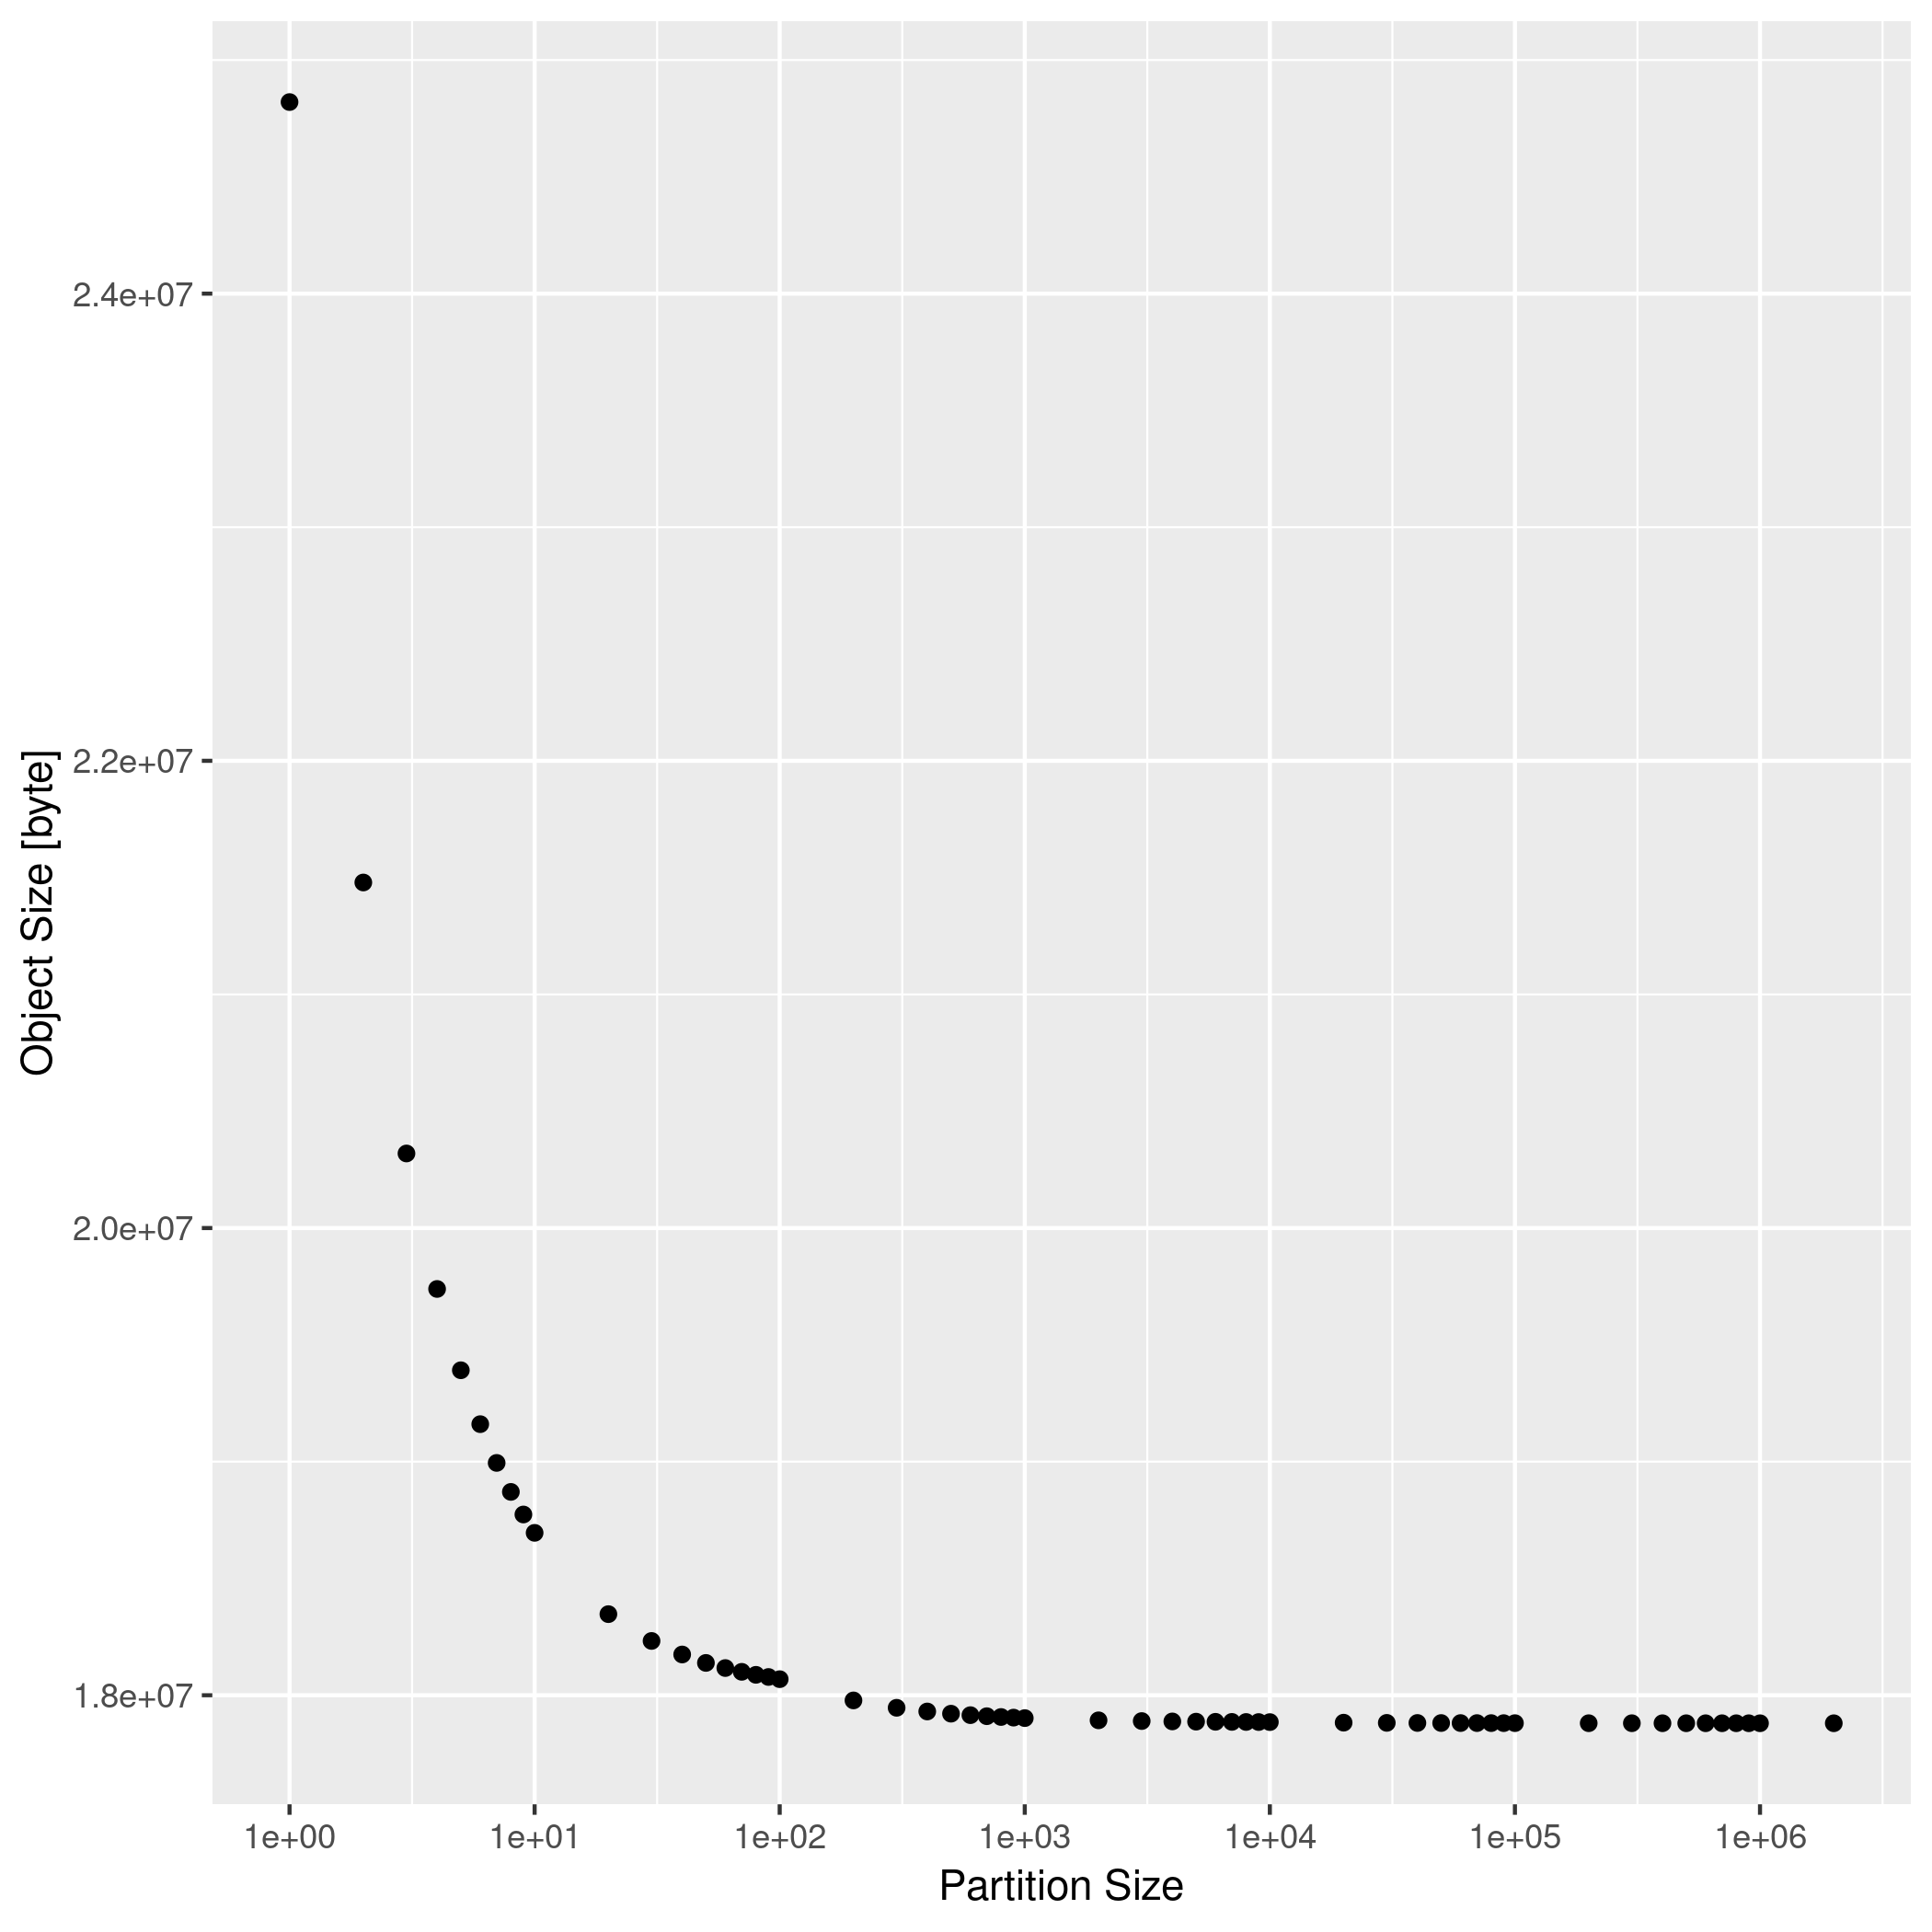
\includegraphics[width=0.9\textwidth]{assets/bench-matvecmult-structured-object-size}
        \label{fig:bench-matvecmult-structured-object-size}}
      \caption{Performance comparison}
    \end{figure}

    // TODO: Linear Minorbreaks in Plots
\section{Summary}
  Advantages: General purpose, good performance, parallel scalability
  Disadv: Static structure (cannot add/remove elements)

OVERALLTODO:
  TODO: ... will be referred to as 'structured matrix' ==== adjacency matrix of structured grids assuming xyz-indexing
\printbibliography
\end{document}
